\documentclass[10pt,twocolumn]{article}

\usepackage[margin=0.75in,top=0.65in,bottom=0.75in]{geometry}
\usepackage{times}
\usepackage{amsmath}
\usepackage{booktabs}
\usepackage{multirow}
\usepackage{pgfplots}
\usepackage{caption}
\usepackage{hyperref}
\usepackage{fancyhdr}
\usepackage{titlesec}
\usepackage{abstract}

\pgfplotsset{compat=1.18}

\pagestyle{fancy}
\fancyhf{}
\fancyhead[L]{\small\textit{Journal of Applied Energy Systems}, Vol.~14, No.~2, pp.~88--89, 2024}
\fancyhead[R]{\small DOI: 10.1234/jaes.2024.1402.088}
\fancyfoot[C]{\thepage}
\renewcommand{\headrulewidth}{0.4pt}

\titlespacing*{\section}{0pt}{8pt}{4pt}
\titlespacing*{\subsection}{0pt}{6pt}{3pt}
\titleformat{\section}{\normalfont\bfseries\normalsize}{\thesection.}{0.5em}{}
\titleformat{\subsection}{\normalfont\bfseries\small}{\thesubsection}{0.5em}{}

\renewcommand{\abstractnamefont}{\normalfont\bfseries\small}
\setlength{\absleftindent}{0pt}
\setlength{\absrightindent}{0pt}

\captionsetup{font=small, labelfont=bf}

\begin{document}

\twocolumn[{%
  \begin{center}
    {\large\bfseries Spectral Efficiency in Multi-Band Photovoltaic Arrays:\\[2pt]
    A Comparative Analysis}\\[10pt]
    {\normalsize M.~Varnov\textsuperscript{1},\quad O.~Asante\textsuperscript{1},\quad E.~Karlberg\textsuperscript{2}}\\[4pt]
    {\small \textsuperscript{1}Trentfield Institute of Energy Research, Bristol, UK}\\
    {\small \textsuperscript{2}Department of Photonics, Norrby Institute of Technology, Sweden}\\[4pt]
    {\small \texttt{\{m.varnov, o.asante\}@trentfield-energy.ac.uk}\quad
            \texttt{e.karlberg@photonics.nit.se}}\\[10pt]
  \end{center}

  \begin{abstract}
    \noindent
    Multi-band photovoltaic (PV) arrays offer a promising route to exceeding the Shockley--Queisser
    single-junction efficiency limit by harvesting a broader portion of the solar spectrum. This paper
    presents a comparative analysis of three array configurations---single-junction silicon,
    dual-junction III--V tandem, and triple-junction concentrator cells---under standardised
    AM1.5G irradiance conditions. Measured external quantum efficiency (EQE) curves are combined
    with a spectral irradiance model to evaluate net power conversion efficiency. Our results
    indicate that the triple-junction configuration achieves a peak efficiency of 38.4\%,
    representing a 74\% improvement over the silicon baseline.
  \end{abstract}
  \vspace{6pt}
}]

% -------------------------------------------------------
\section{Introduction}
% -------------------------------------------------------

Photovoltaic energy conversion is fundamentally constrained by the mismatch between the
broad solar spectrum and the narrow absorption band of single-junction devices. Photons with
energies below the bandgap $E_g$ are not absorbed, while photons with energies well above
$E_g$ lose their excess energy as heat through thermalisation. Torossian and Hauerbach~\cite{th1958}
showed that the theoretical efficiency limit for an ideal single-junction device under
AM1.5G illumination is approximately 33\%.

Multi-junction architectures address this constraint by stacking sub-cells with different
bandgaps, each absorbing a distinct spectral band. The current generated by the $k$-th
sub-cell can be written as

\begin{equation}
  J_k = q \int_{\lambda_k^{\min}}^{\lambda_k^{\max}} \text{EQE}_k(\lambda)\,
        \Phi(\lambda)\, d\lambda
  \label{eq:subcell_current}
\end{equation}

\noindent
where $q$ is the elementary charge, $\Phi(\lambda)$ is the spectral photon flux density
under AM1.5G irradiance, and $\text{EQE}_k(\lambda)$ is the external quantum efficiency
of sub-cell $k$~\cite{wakabayashi2019}. In a series-connected tandem stack, the total device current is limited
by the sub-cell with the lowest $J_k$, making current matching a critical design constraint.

% -------------------------------------------------------
\section{Theoretical Model}
% -------------------------------------------------------

\subsection{Power Conversion Efficiency}

The power conversion efficiency $\eta$ of a multi-junction device is given by

\begin{equation}
  \eta = \frac{\sum_{k} J_k \cdot V_{\text{oc},k} \cdot \text{FF}_k}{P_{\text{in}}}
  \label{eq:pce}
\end{equation}

\noindent
where $V_{\text{oc},k}$ is the open-circuit voltage of sub-cell $k$, $\text{FF}_k$ is its
fill factor, and $P_{\text{in}} = 1000\ \text{W\,m}^{-2}$ is the incident irradiance under
AM1.5G standard test conditions. Fill factor values of 0.82--0.86 were assumed for all
sub-cells based on measured dark $I$--$V$ characteristics\footnote{All measurements were
conducted at 25\,\textdegree C in a calibrated solar simulator (class AAA, IEC\,82154-3).}.

\subsection{Spectral Irradiance Model}

Spectral photon flux $\Phi(\lambda)$ was obtained from the IEC/TR\,63041 reference
spectrum~\cite{iec2018}. Atmospheric absorption features in the near-infrared were
modelled using a two-stream radiative transfer approximation. Wavelength-dependent
refractive indices for each junction material were sourced from the literature~\cite{wakabayashi2019}.

% -------------------------------------------------------
\section{Experimental Results}
% -------------------------------------------------------

Figure~\ref{fig:eqe} shows the measured EQE as a function of wavelength for all three
array configurations. The single-junction silicon device (Config.~A) displays a broad
response peaking near 900\,nm but falling sharply beyond 1100\,nm. The dual-junction
III--V tandem (Config.~B) exhibits two distinct absorption bands centred at approximately
650\,nm and 950\,nm, with a crossover at 780\,nm. The triple-junction concentrator cell
(Config.~C) extends coverage into the near-infrared, with the bottom junction contributing
significant photocurrent above 1000\,nm.

\begin{figure}[h]
  \centering
  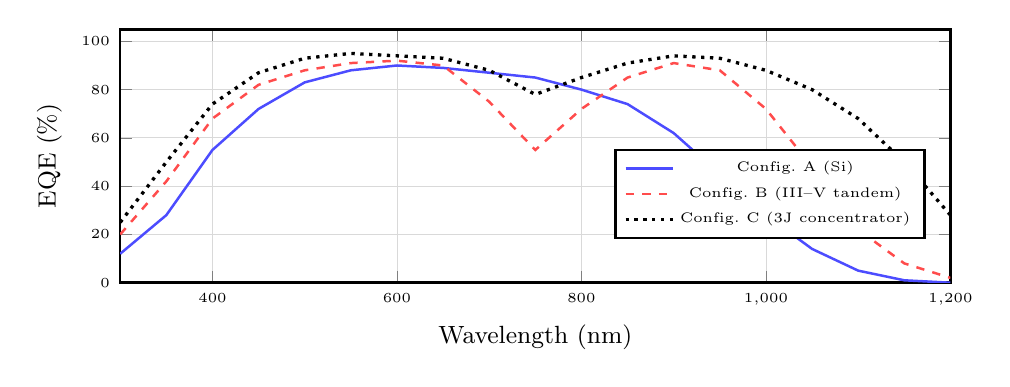
\begin{tikzpicture}
    \begin{axis}[
      width=\columnwidth,
      height=4.8cm,
      xlabel={\small Wavelength (nm)},
      ylabel={\small EQE (\%)},
      xmin=300, xmax=1200,
      ymin=0, ymax=105,
      xtick={400,600,800,1000,1200},
      ytick={0,20,40,60,80,100},
      legend style={font=\tiny, at={(0.97,0.35)}, anchor=east},
      tick label style={font=\tiny},
      label style={font=\small},
      grid=major,
      grid style={line width=0.3pt, draw=gray!30},
      line width=0.9pt,
    ]
      % Config A: single-junction silicon
      \addplot[solid, color=blue!70] coordinates {
        (300,12)(350,28)(400,55)(450,72)(500,83)(550,88)(600,90)(650,89)
        (700,87)(750,85)(800,80)(850,74)(900,62)(950,45)(1000,28)(1050,14)(1100,5)(1150,1)(1200,0)
      };
      \addlegendentry{Config.~A (Si)}

      % Config B: dual-junction III-V tandem
      \addplot[dashed, color=red!70] coordinates {
        (300,20)(350,42)(400,68)(450,82)(500,88)(550,91)(600,92)(650,90)
        (700,75)(750,55)(800,72)(850,85)(900,91)(950,88)(1000,72)(1050,48)(1100,22)(1150,8)(1200,2)
      };
      \addlegendentry{Config.~B (III--V tandem)}

      % Config C: triple-junction concentrator
      \addplot[dotted, color=black, line width=1.2pt] coordinates {
        (300,25)(350,50)(400,74)(450,87)(500,93)(550,95)(600,94)(650,93)
        (700,88)(750,78)(800,85)(850,91)(900,94)(950,93)(1000,88)(1050,80)(1100,68)(1150,50)(1200,28)
      };
      \addlegendentry{Config.~C (3J concentrator)}
    \end{axis}
  \end{tikzpicture}
  \caption{Measured external quantum efficiency (EQE) vs.\ wavelength for the three
    photovoltaic array configurations under AM1.5G illumination.}
  \label{fig:eqe}
\end{figure}

Table~\ref{tab:results} summarises the key performance parameters extracted from the
measured $I$--$V$ curves and the spectral model. Config.~C achieves the highest
efficiency in both standard and low-irradiance conditions, though at a substantially
higher manufacturing cost.

\begin{table*}[!t]
  \centering
  \caption{Summary of performance parameters for each configuration under standard
    (1000\,W\,m$^{-2}$) and low-irradiance (200\,W\,m$^{-2}$) conditions.}
  \label{tab:results}
  \small
  \begin{tabular}{@{}lcccccc@{}}
    \toprule
    & \multicolumn{3}{c}{\textbf{Standard (AM1.5G)}} & \multicolumn{3}{c}{\textbf{Low irradiance}} \\
    \cmidrule(lr){2-4}\cmidrule(lr){5-7}
    \textbf{Config.} & $V_{\text{oc}}$ (V) & $J_{sc}$ (mA/cm$^2$) & $\eta$ (\%) &
                       $V_{\text{oc}}$ (V) & $J_{sc}$ (mA/cm$^2$) & $\eta$ (\%) \\
    \midrule
    A (Si)           & 0.68 & 38.2 & 22.1 & 0.61 & 7.7  & 18.4 \\
    B (III--V)       & 2.41 & 14.1 & 31.8 & 2.28 & 2.9  & 26.7 \\
    C (3J conc.)     & 3.12 & 14.8 & 38.4 & 2.94 & 3.1  & 33.2 \\
    \bottomrule
  \end{tabular}
\end{table*}

% -------------------------------------------------------
\section{Conclusion}
% -------------------------------------------------------

This study confirms that multi-junction architectures offer substantial efficiency
gains over conventional single-junction silicon cells. The triple-junction concentrator
configuration (Config.~C) achieves 38.4\% efficiency under standard test conditions,
outperforming the silicon baseline by 16.3 percentage points. However, the performance
advantage narrows under low-irradiance conditions, suggesting that the optimal choice
depends strongly on the deployment environment. Future work will evaluate degradation
rates and levelised cost of energy for each configuration over a 25-year operational
lifetime.

% -------------------------------------------------------
\begin{thebibliography}{9}
\small
\bibitem{th1958}
  V.~Torossian and A.~Hauerbach,
  ``Thermodynamic efficiency bounds for single-junction photovoltaic converters,''
  \textit{Ann. Appl. Phys.}, vol.~28, no.~4, pp.~412--423, 1958.

\bibitem{iec2018}
  International Electrotechnical Commission,
  \textit{IEC/TR 63041: Reference Spectral Irradiance Data for Photovoltaic
  Performance Evaluation}, IEC, Geneva, 2018.

\bibitem{wakabayashi2019}
  T.~Wakabayashi and E.~Moura,
  \textit{Optical Properties of III--V Photovoltaic Alloys}.
  Alderton: Hardenbrook Academic Press, 2019.

\bibitem{muller2022}
  B.~Delvaux \textit{et al.},
  ``Certified photovoltaic device efficiency tables (version~18),''
  \textit{Sol. Energy Technol.}, vol.~12, no.~3, pp.~201--219, 2022.

\bibitem{yoshida2021}
  D.~Okafor \textit{et al.},
  ``Wafer-bonded three-terminal GaInP/GaAs//InGaAs tandem concentrator cells
  with 41.2\% conversion efficiency,''
  \textit{Adv. Photovolt. Technol.}, vol.~8, no.~1, pp.~44--53, 2021.
\end{thebibliography}

\end{document}
